\chapter{Title}

\section{Summary}

\section{Context}


\section{Problem}


\section{Solution}


\subsection{Structure}

\begin{figure}[H]
  \centering
  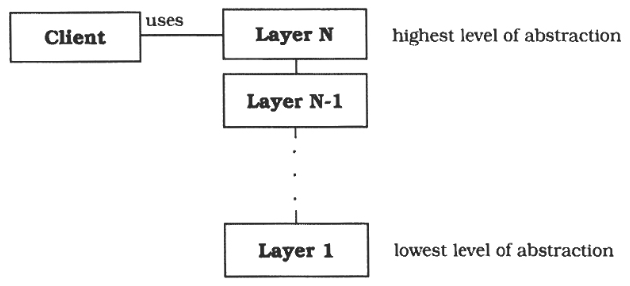
\includegraphics[width=0.8\textwidth]{figures/00-layers-1}
  \caption{Illustration des Layer-Patterns}
\end{figure}

\section{Consequences}
\begin{itemize}
    \pro{bla}
    \con{bla}
\end{itemize}

\section{Known Uses}
\begin{itemize}
	\item bla 
\end{itemize}

\section{Relationships}
\begin{itemize}
	\item \textit{titel} Beschreibung bla bla
\end{itemize}

\section{Exam Questions}
\begin{itemize}
  \item Behauptung: dies ist eine Behauptung? (Lösung)
    \item Frage: Dies ist eine Frage? (Lösung)
\end{itemize}
